\section{Zielsetzung}
Im Versuch wird das Emissionsspektrum einer Kupferröntgenröhre und die Absorptionsspektren
verschiedener anderer Stoffe untersucht.

\section{Theorie}
\subsection{Entstehung von Röntgenstrahlung}
Wenn beschleunigte Elektronen mit Materie wechselwirken, so entsteht Röntgenstrahlung.
Die Beschleunigung der Elektronen geschieht im Versuch mit einer Röntgegnröhre,
in der Elektronen mittels des Glühelektrischeneffekts aus einer Kathode ausgelöst werden
und dann zu einer Anode hin bechleunigt werden.
Treffen die Elektronen auf das Anodenmaterial, so entsteht Röntgenstrahlung auf zwei
verschiedene Arten.


1. Bremsstrahlung: Durch die Wechselwirkung der Elektronen mit dem Coulombfeld der
Atomkerne des Anodenmaterials, werden die Elektronen abgebremst. Durch den Abbremsvorgang
verliert das Elektron an Energie, die in Form eines Photons emittiert wird.
Dabei entsteht ein kontinuierliches Spektrum, das eine Grenzwellenlänge aufweist,
unter der keine Röntgenstrahlung mehr gemessen werden kann:
\begin{align*}
  \lambda_{\symup{min}} = \frac{hc}{e_0 U}
\end{align*}
Hierbei ist $h$ das Plancksche Wirkungsquantum, $c$ die Vakuumlichtgeschwindigkeit,
$e_0$ die Elektronenruhemasse und $U$ die Beschleunigungsspannung.
Die minimale Wellenlänge ergibt sich aus der vollständigen Abbremsung des Elektrons,
bei der die gesamte kinetische Energie des Elektrons, die aus der Beschleunigung
gewonnen wurde, umgewandelt wird.
Das dabei entstehende kontinuierliche Spektrum wird Bremsspektrum oder als Bremsberg
bezeichnet.


2. Charakteristisches Spektrum: Bei der Entstehung des charakteristischen Spektrums
schlagen die beschleunigten Elektronen, Elektronen aus den tieferen Schalen der Anodenatome
heraus. In die entstandene Lücke rückt ein Atom aus einer höheren Schale in diese Schale
runter und emittiert dabei ein Röntgenquant. Die dabei freiwerdenden Energie ergibt sich aus
dern Differenz zwischen Urpsrungsniveau und Zielniveau.
Die Bindungenergie einer Elektronenschale ergibt sich aus folgender Beziehung:
\begin{align*}
  E_n = - R_{\infty}~z_{\symup{eff}}^2~\frac{1}{n^2}
\end{align*}
Dabei ist $R_\infty$ die Rydbergenergie mit $\SI{13,6}{\eV}$. Die Konstante $z_{\symup{eff}} = z - \sigma$
beschreibt die effektive Kernladung, die sich aus der Differenz zwischen der tatsächlichen
Kernladung $z$ und der Abschirmkonstante $\sigma$ ergibt.
Es ergibt sich ein diskretes Spektrum. Die scharf abgegrenzten Linien des Röntgenspektrums
werden mit $K_{\alpha}, K_{\beta}, L_{\alpha}$ usw. bezeichnet. Der Großbuchstabe beschreibt
hier auf welche Schale das Elektron fällt, der griechische Buchstabe, um wieviele Schalen
höher es sich zuvor befand.
Die Abschirmkonstante ist für jedes Elektron in der äußeren Schale unterschiedlich,
weshalb sich für jedes Elektron unterschiedliche Bindungsenergien ergeben, was dazu führt,
dass jede Linie im charakteristischen Spektrum aus kleinen, sehr nah beieinander liegenden
Linien besteht. Diese Linien werden als Feinstruktur bezeichnet und werden dem Bremsspektrum aufgesetzt,
wie in Abbildung \ref{abb1a} zu sehen ist.

\subsection{Absorption von Röntgenstrahlung}
Bei der Wechselwirkung von Röntgenstrahlen mit einer Energie unter $\SI{1}{\mega \eV}$
spielen zwei Effekte eine wichtige Rolle: Zum einen der Compton-Effekt und zum anderen
der Photoeffekt. Die Compton-Streuung ist vor allem bei Absorbern mit wenigen Elektronen
von Bedeutung. Die einstrahlenden Röntgenquanten treffen auf die Hüllenelektronen der
Absorberatome, wobei sie mit einer gewissen Wahrscheinlichkeit absorbiert werden.
Die Absorptionswahrscheinlichkeit ist hier umgekehrt proportional zur Energie der einfallenden
Röntgenquanten. Erreichen die Röntgenquanten die Bindungsenergie der Elektronen, so können sie diese ionisieren.
Die Absorptionswahrscheinlichkeit steigt sprunghaft an. Diese Kanten werden Absorptionskanten
genannt und erhalten in der Nomenklatur den Buchstaben der ionisierten Schale. Ein Absorptionsspektrum
mit Absorptionskanten ist in Abbildung \ref{abb1b} zu sehen.
\FloatBarrier
\begin{figure}
  \centering
  \begin{subfigure}{.4\textwidth}
    \centering
  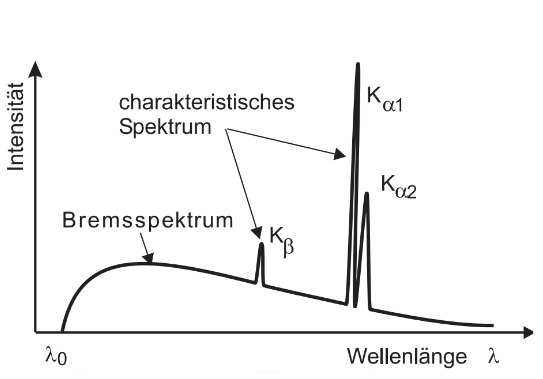
\includegraphics[scale=0.3]{b1.PNG}
  \caption{Emissionsspektrum \cite{Q1}}
  \label{abb1a}
\end{subfigure}
\begin{subfigure}{.4\textwidth}
  \centering
 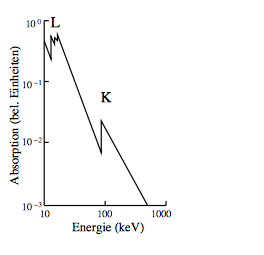
\includegraphics[scale=0.6]{b2.PNG}
 \caption{Absorptionsspektrum \cite{Q1}}
 \label{abb1b}
 \end{subfigure}
 \caption{Emissions- und Absorptionsspektren von Röntgenstrahlung.}
 \label{abb1}
\end{figure}
\FloatBarrier
Auch bei der Absorption von Röntgenstrahlung muss die Feinstruktur beachtet werden.
Somit ergibt sich mit der Sommerfeldschen Feinstrukturformel die Bindungsenergie für
ein Elektron, das sich in einer Schale mit der Feinstruktur befindet:
\begin{align*}
  E_{n,j} = - R_\infty \left( z_{\symup{eff,1}}^2 ~\frac{1}{n^2}+\alpha^2~z_{\symup{eff,2}}^4~\frac{1}{n^3} ~\left(\frac{1}{j + 1/2} - \frac{3}{4n}\right) \right)
\end{align*}
In der Formel steht $n$ für die Hauptquantenzahl, $j$ für die Gesamtdrehimpulsquantenzahl, und $\alpha$ für die
Sommerfeldsche Feinstrukturkonstante.
Die Bestimmung der Abschirmkonstanten $\sigma$ erfolgt aus der Energiedifferenz zweier Feinstrukturkonstanten:
\begin{align}
  \label{eq:quecksilber}
  \sigma_L = Z -\left(\frac{4}{\alpha} \sqrt{\frac{\Delta E_L}{R_\infty}}-\frac{5 \Delta E_L}{R_\infty}\right)^{1/2} \left(1 + \frac{19}{32}~\alpha^2 ~\frac{\Delta E_L}{R_\infty}\right)^{1/2}
\end{align}
Hier gibt $\Delta E_L = E_{L_2} - E_{L_3}$, die Energiedifferenz zwischen den Schalen $L_2$ und $L_3$ an.
\FloatBarrier
\subsection{Bragg-Gleichung}
Die Bragg-Reflexion wird zur Bestimmung der Wellenlänge der Röntgenstrahlung verwendet. Dafür muss die
Strahlung auf einen kristall mit regelmäßiger Gitterstruktur gerichtet werden. Treffen die Röntgenstrahlen
auf eine solche Gitterstruktur, werden sie gebeugt und reflektieren miteinander. Unter einem bestimmten Winkel
$\Theta$ kommt es zu konstruktiver Interferenz. Der Winkel $\Theta$ wird als Glanzwinkel bezeichnet.
Mit der Gitterkonstanten $d$ und der Beugungsordnung $n$ ergibt sich die Bragg-Bedingung:
\begin{equation}\label{eq1}
  2d \sin(\Theta) = n~\lambda
\end{equation}
In Abbildung \ref{abb2} ist die Photonenbeugung am Gitter schematisch dargestellt.
\FloatBarrier
\begin{figure}
  \centering
  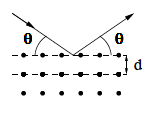
\includegraphics[scale=0.7]{b3.PNG}
  \caption{Veranschaulichung der Bragg-Bedingung für die Photonenbeugung am Gitter. \cite{Q1}}
  \label{abb2}
\end{figure}

\section{Durchführung}
Zur Durchführung des Versuchs ist ein Geiger-Müller-Zählrohr,
ein Lithiumfluorid-Kristall (LiF-Kristall), sowie eine Kupfer-Röntgenröhre zur Aussendung von röntgenstrahlung verwendet.
Vor dem Geiger-Müller-Zählrohr können Träger mit Absorbern verschiedener Elemente befestigt werden.
Die einzelnen Ansteuerungen werden elektronisch über einen Rechner geregelt.
Im ersten Teil des Versuchs wird die Bragg-Bedingung überprüft. Dafür wird der Winkel des LiF-Kristalls
fest auf $\SI{14}{\degree}$ eingestellt und mit dem Geiger-Müller-Zählrohr ein Winkelbereich
von $\SI{26}{\degree}$ bis $\SI{30}{\degree}$ in $\SI{0,1}{\degree}$ Schritten abgefahren. In dem enstandenen Graph werden
dann Bremsberg, $K_{\alpha}$ und $K_{\beta}$ identifiziert und beschriftet. Das erhaltenen Maximum wird
mit dem Theoriewert aus Gleichung \ref{eq1} verglichen.

\noindent Im zweiten Teil des Versuchs wird das Emissionsspektrum der Röntgenröhre ermittelt. Dazu wird der Kristall
Im Koppelmodus 2:1 von $\SI{4}{\degree}$ bis $\SI{26}{\degree}$ in $\SI{0,2}{\degree}$ Schritten umfahren.
Die Intensität wird für $\SI{5}{\sec}$ gemessen.

\noindent Im dritten Teil des Versuchs werden die Absorptionsspektren verschiedener Absorber ermittelt und analysiert.
Dies geschieht, indem jeweils ein Träger mit einem Absorber vor das Geiger-Müller-Zählror gespannt wird und
der Kristall in $\SI{0,1}{\degree}$ Schritten umfahren wird. Für jeden Winkel wird dann für $\SI{20}{\sec}$ die Intensität
der Röntgenstrahlen gemessen. Die Winkel, die das Geiger-Müller-Zählrohr bei den verschiedenen Absorbern
abfahren muss, ist materialspezifisch und wurde vorher berechnet.
Zunächst werden die Absorptionsspektren von drei verschiedenen Elementen, deren Ordnungszahlen zwischen 30 und 50 liegen
untersucht und im Anschluss ein Absorber, dessen Orsnungszahl über 70 liegt.
Für die ersten drei Absorber sollen die Energieübergänge und daraus die Abschirmkonstanten der $K$-Kanten bestimmt werden,
für den letzten Absorber werden die Energieübergänge und die Abschirmkonstanten der $L$-Kanten bestimmt.

\section{Auswertung}

\subsection{Überprüfen der Bragg-Bedingung}
Zur Überprüfung der Bragg-Bedingung wird das Maximum der Messung aus Abbildung \ref{abb:1} abgelesen und mit dem Literaturwert
von $\theta = \SI{14}{\degree}$ verglichen. Das Maximum aus Abbildung \ref{abb:1} liegt bei $\theta_{\symup{gemessen}} = \SI{14,2}{\degree}$,
somit ist die Bragg-Bedingung erfüllt.
\begin{figure}
  \centering
  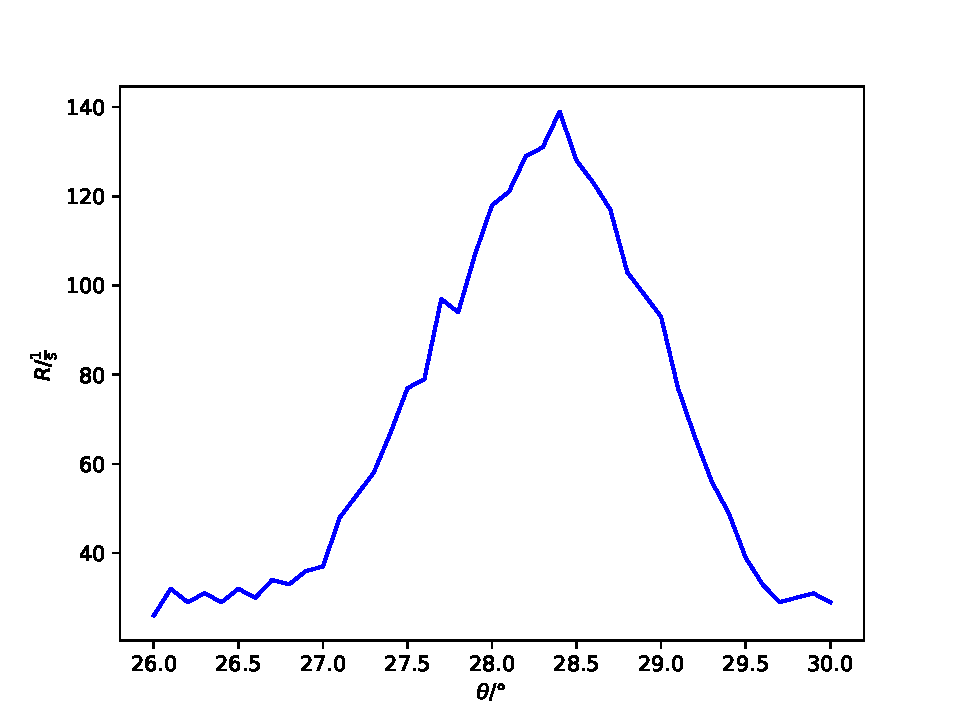
\includegraphics[scale= 0.7]{Plot1.pdf}
  \caption{Überprüfung der Bragg-Bedingung, Rate $R$.}
  \label{abb:1}
\end{figure}

\subsection{Das Emissionsspektrum einer Cu-Röntgenröhre}
In Abbildung \ref{abb:2} ist das Emissionspektrum einer Cu-Röntgenröhre dargestellt. Das Bremsspektrum ist dabei das gesamte Spektrum,
die $K_{\symup{\alpha}}$-Linie befindet sich bei $\theta_{K_{\symup{\alpha}}} = \SI{20,0}{\degree}$ und die $K_{\symup{\beta}}$-Linie
befindet sich bei $\theta_{K_{\symup{\beta}}} = \SI{22,2}{\degree}$.
In Abbildung \ref{abb:kupferzoom} ist der Anfangsbereich des Bremsspektrum noch einmal genauer dargestellt, hieraus lässt sich der
Grenzwinkel $\theta_{\symup{min}} = \SI{5}{\degree}$ ablesen. Die zugehörige maximale Energie lässt sich durch die Formel
\begin{equation}
  \label{eq:energie}
  E = c \nu = \frac{c h}{\lambda} = \frac{c h}{2d \sin(\theta)}
\end{equation}
berechnen, mit $d= \SI{201,4}{\pico\meter}$, $c$ der Lichtgeschwindigkeit und $h$ dem Planckschen Wirkungsquantum. Daraus folgt für die maximale Energie und
aus der Braggbedingung die minimale Wellenlänge $\lambda_{\symup{min}}$
\begin{align*}
  E_{\symup{max}} = \SI{35,317}{\kilo\eV} \\
  \lambda_{\symup{min}} = \SI{35,1}{\pico\meter}
\end{align*}
Die Abschirmkonstanten $\sigma_1 $, $\sigma_2$ und $\sigma_3$ kann somit aus der Formeln
\begin{align}
  E_{\symup{k, abs}} = R_{\symup{\infty}} (z-\sigma_1)² \\
  E_{\symup{k, \alpha}} = R_{\symup{\infty}} (z-\sigma_1)²-R_{\symup{\infty}} \frac{1}{4} (z-\sigma_2)² \\
  E_{\symup{k, \alpha}} = R_{\symup{\infty}} (z-\sigma_1)²-R_{\symup{\infty}} \frac{1}{9} (z-\sigma_3)²
\end{align}
bestimmt werden. Mit $Z_{\symup{Kupfer}} = 29$ und $R_{\symup{\infty}} = \SI{13,6}{\eV}$ und den aus den Winkeln berechneten Energien für die $K_{\symup{\alpha}}$- und für die
$K_{\symup{\beta}}$-Kante mit Hilfe der Formel \eqref{eq:energie}
\begin{align*}
  \theta_{\symup{\alpha}} &= \SI{20,0}{\degree} \\
  \theta_{\symup{\beta}} &= \SI{22,2}{\degree} \\
  E_{\symup{\theta_{\symup{\alpha}}}} &= \SI{8,146}{\kilo\eV} \\
  E_{\symup{\theta_{\symup{\beta}}}} &= \SI{8,999}{\kilo\eV}
\end{align*}
lässt sich somit die Abschirmkonstanten berechnen
\begin{align*}
  \sigma_1 =  3,30  \\
  \sigma_2 =  13,31  \\
  \sigma_3 =  29
\end{align*}
Die Bestimmung der Halbwärtsbreite der Peaks ist in Abbildung \ref{abb:peak1} und \ref{abb:peak2} veranschaulicht. Hieraus erhalten
wir die Werte $d_1=\SI{0,64}{\degree}$ und $d_2=\SI{0,78}{\degree}$. Die Daraus berechneten Energien sind
\begin{align*}
  E_{\symup{d1}} = \SI{63,57}{\eV} \\
  E_{\symup{d2}} = \SI{60,618}{\eV}
\end{align*}
Das Auflösungsvermögen beschreibt in der Physik das Maß für den geringsten Abstand
zweier Messobjekte, die von der Messapparatur mit Sicherheit noch getrennt aufgelöst
bzw. gemessen werden können. In der Optik ist zum Beispiel das Maß für den gerings-
te Abstand, der aufgelöst werden kann, wenn das Intensitätsmaximum eines Objektes
auf dem ersten Intensitätsminimum des anderen Objektes liegt. Wird dieser Abstand
geringer, lassen sich beide Objekte nicht mehr sauber voneinander trennen.
\begin{figure}
  \centering
  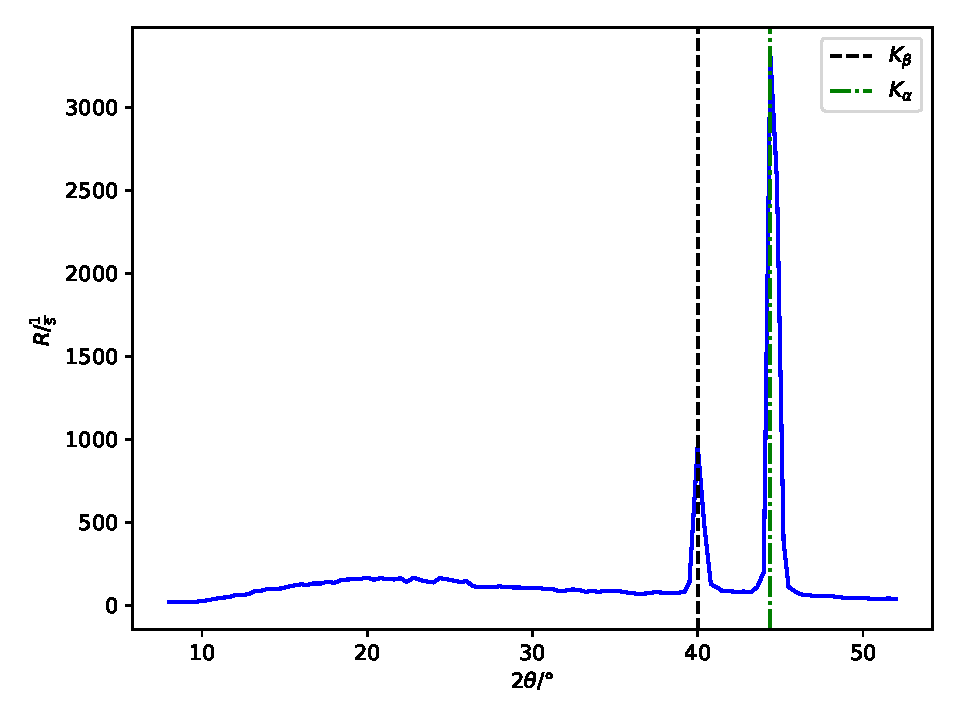
\includegraphics[scale = 0.7]{Kupfer.pdf}
  \caption{Emissionsspektrum einer Cu-Röntgenröhre, Rate $R$.}
  \label{abb:2} %Kupfer
\end{figure}
\begin{figure}
  \centering
  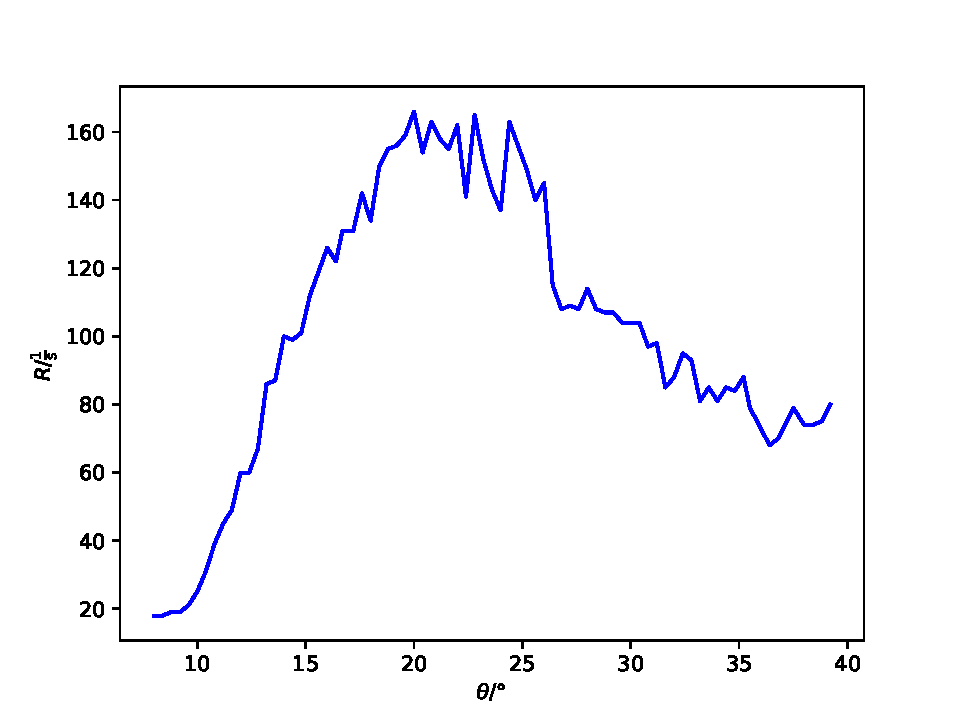
\includegraphics[scale = 0.7]{PlotProbe.pdf}
  \caption{Anfangsbereich des Bremsspektrums von Kupfer, Rate $R$.}
  \label{abb:kupferzoom} %Kupferzoom
\end{figure}
\begin{figure}
  \centering
  \includegraphics[scale = 0.7]{Halbwärtsbreite.pdf}
  \caption{Messung der Halbwärtsbreite des $K_{\symup{\beta}}$-Peaks, Rate $R$.}
  \label{abb:peak1} %Peak1
\end{figure}
\begin{figure}
  \centering
  \includegraphics[scale = 0.7]{Halbwärtsbreite2.pdf}
  \caption{Messung der Halbwärtsbreite des $K_{\symup{\alpha}}$-Peaks, Rate $R$.}
  \label{abb:peak2} %Peak2
\end{figure}
\begin{table}
  \centering
  \caption{Messwerte zum Emissionspektrum einer Cu-Röntgenröhre, Rate $R$.}
  \label{tab:1}
  \begin{tabular}{c c | c c | c c}
    \toprule
    $\theta$ / $\si{\degree}$ & $R$ / $\si{\per\second}$ & $\theta$ / $\si{\degree}$ & $R$ / $\si{\per\second}$ & $\theta$ / $\si{\degree}$ & $R$ / $\si{\per\second}$ \\
    \midrule
    8.00 & 18.00 & 22.80 & 165.00 & 37.50 & 79.00 \\
    8.40 & 18.00 & 23.20 & 152.00 & 38.00 & 74.00 \\
    8.80 & 19.00 & 23.60 & 143.00 & 38.40 & 74.00 \\
    9.20 & 19.00 & 24.00 & 137.00 & 38.80 & 75.00 \\
    9.60 & 21.00 & 24.40 & 163.00 & 39.20 & 80.00 \\
    10.00 & 25.00 & 24.80 & 156.00 & 39.50 & 136.00 \\
    10.40 & 31.00 & 25.20 & 149.00 & 40.00 & 960.00 \\
    10.80 & 39.00 & 25.60 & 140.00 & 40.40 & 485.00 \\
    11.20 & 45.00 & 26.00 & 145.00 & 40.80 & 127.00 \\
    11.60 & 49.00 & 26.40 & 115.00 & 41.20 & 105.00 \\
    12.00 & 60.00 & 26.80 & 108.00 & 41.50 & 85.00 \\
    12.40 & 60.00 & 27.20 & 109.00 & 42.00 & 84.00 \\
    12.80 & 67.00 & 27.60 & 108.00 & 42.40 & 79.00 \\
    13.20 & 86.00 & 28.00 & 114.00 & 42.80 & 83.00 \\
    13.60 & 87.00 & 28.40 & 108.00 & 43.20 & 77.00 \\
    14.00 & 100.00 & 28.80 & 107.00 & 43.60 & 108.00 \\
    14.40 & 99.00 & 29.20 & 107.00 & 44.00 & 198.00 \\
    14.80 & 101.00 & 29.60 & 104.00 & 44.40 & 3314.00 \\
    15.20 & 112.00 & 30.00 & 104.00 & 44.80 & 2555.00 \\
    15.60 & 119.00 & 30.40 & 104.00 & 45.20 & 386.00 \\
    16.00 & 126.00 & 30.80 & 97.00 & 45.50 & 111.00 \\
    16.40 & 122.00 & 31.20 & 98.00 & 46.00 & 76.00 \\
    16.70 & 131.00 & 31.60 & 85.00 & 46.40 & 61.00 \\
    17.20 & 131.00 & 32.00 & 88.00 & 46.80 & 59.00 \\
    17.60 & 142.00 & 32.40 & 95.00 & 47.20 & 54.00 \\
    18.00 & 134.00 & 32.80 & 93.00 & 47.60 & 56.00 \\
    18.40 & 150.00 & 33.20 & 81.00 & 48.00 & 57.00 \\
    18.80 & 155.00 & 33.60 & 85.00 & 48.40 & 50.00 \\
    19.20 & 156.00 & 34.00 & 81.00 & 48.80 & 46.00 \\
    19.60 & 159.00 & 34.40 & 85.00 & 49.20 & 45.00 \\
    20.00 & 166.00 & 34.80 & 84.00 & 49.60 & 45.00 \\
    20.40 & 154.00 & 35.20 & 88.00 & 50.00 & 43.00 \\
    20.80 & 163.00 & 35.50 & 79.00 & 50.40 & 40.00 \\
    21.20 & 158.00 & 36.00 & 73.00 & 50.80 & 35.00 \\
    21.60 & 155.00 & 36.40 & 68.00 & 51.20 & 39.00 \\
    22.00 & 162.00 & 36.80 & 70.00 & 51.60 & 41.00 \\
    22.40 & 141.00 & 37.20 & 75.00 & 52.00 & 36.00 \\
    \bottomrule
  \end{tabular} %Tabelle Messwerte Kupfer
\end{table}

\newpage

\subsection{Absorptionsspektrum von leichten Elementen}
Die K-Kanten des Absorptionsspektrums lassen sich aus den Abbildungen \ref{abb:brom}, \ref{abb:strontium} und \ref{abb:zirconium} ablesen
\begin{align*}
  \theta_{\symup{Brom}} &= \SI{23,05}{\degree} \\
  \theta_{\symup{Strontium}} &= \SI{11,35}{\degree} \\
  \theta_{\symup{Zirconium}} &= \SI{9,65}{\degree}
\end{align*}
Aus den Winkeln folgt für die Energie nach Formel \eqref{eq:energie}
\begin{align*}
  E_{\symup{Brom}} &= \SI{13,632}{\kilo\eV} \\
  E_{\symup{Strontium}} &= \SI{15,640}{\kilo\eV} \\
  E_{\symup{Zirconium}} &= \SI{18,362}{\kilo\eV}
\end{align*}
Aus der Gleichung
\begin{equation}
  \label{eq:zquadrat}
  E_n = -R_{\infty} z²_{\symup{eff}} \cdot \frac{1}{n²}
\end{equation}
kann man die Formeln für $\sigma_{\symup{K}}$ aufstellen, mit der Annahme, dass $E_{\symup{K}} = E_{\symup{\beta}}$ gilt.
\begin{align}
  \sigma_{\symup{K}} &= z-\sqrt{\frac{E_{\symup{\beta}}}{R_{\symup{\infty}}}}
\end{align}
Mit den Energien und den Ordnungszahlen $Z_{\symup{Brom}}=35$, $Z_{\symup{Strontium}}=38$ und $Z_{\symup{Zirconium}}=40$  folgt für die Abschirmungskonstanten
\begin{align*}
  \sigma_{\symup{K_{Brom}}} &=  3,340 \\
  \sigma_{\symup{K_{Strontium}}} &=  4,088 \\
  \sigma_{\symup{K_{Zirconium}}} &=  3,255
\end{align*}
Nach Mosley ist die Energie $E_{\symup{K}}$ proportional zu $z²$. Dazu soll nun eine linerare Regression der Form
\begin{equation}
  \label{eq:lineare_Regression}
  \sqrt{E_{\symup{K}}} = m \cdot z +b
\end{equation}
durchgeführt werden. In Abbildung \ref{abb:lineare_Regression} ist diese Lineare Regression dargestellt, aus dieser ergeben sich die Werte
der Steigung $m$ und des y-Achsenabschnittes $b$
\begin{align*}
  m &= \num{1.47(27)e-9} \, \sqrt{\symup{J}} \\
  b &= \num{-0.5(10)e-8} \, \sqrt{\symup{J}}
\end{align*}
Der Vergleich der lineare Regression mit der Formel \eqref{eq:zquadrat} führt zu dem Wert der Rydbergenergie
\begin{equation}
  R_{\symup{\infty berechnet}} = m² = \SI{13(5)}{\eV}
\end{equation}

\begin{figure}
  \centering
  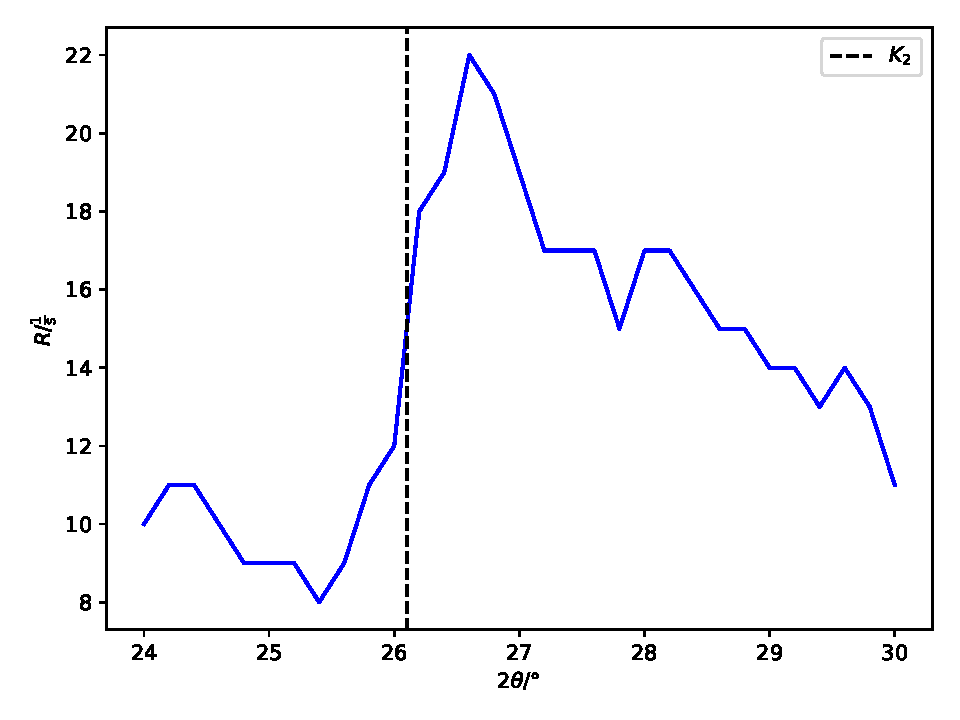
\includegraphics[scale=0.7]{Brom.pdf}
  \caption{Absorptionsspektrum von Brom, Rate $R$.}
  \label{abb:brom} %Brom
\end{figure}
\begin{figure}
  \centering
  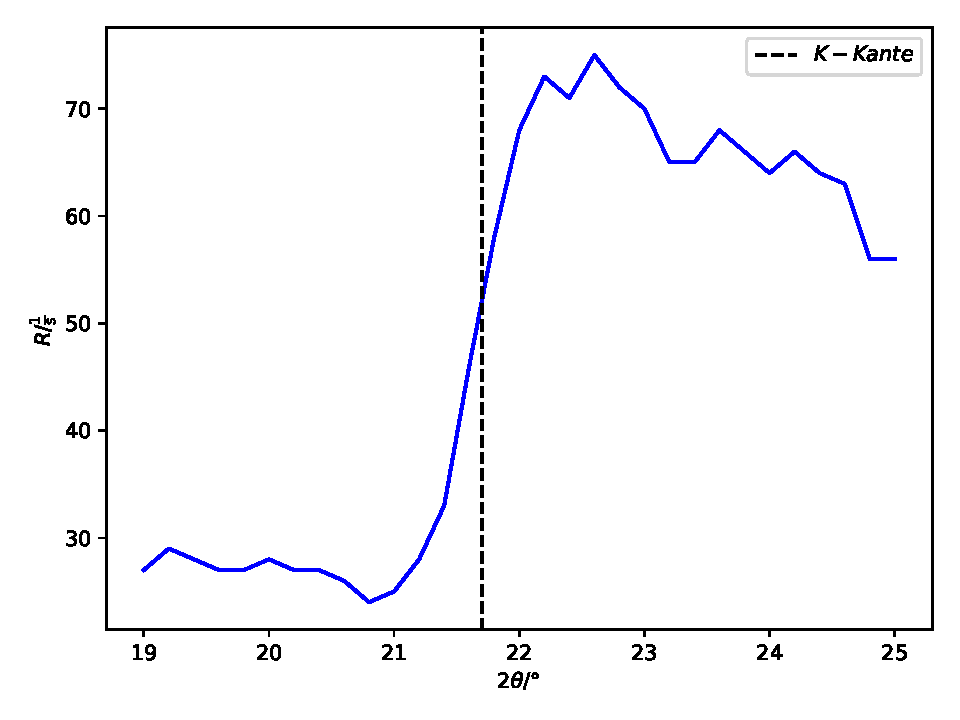
\includegraphics[scale=0.7]{Strontium.pdf}
  \caption{Absorptionsspektrum von Strontium, Rate $R$.}
  \label{abb:strontium} %Strontium
\end{figure}
\begin{figure}
  \centering
  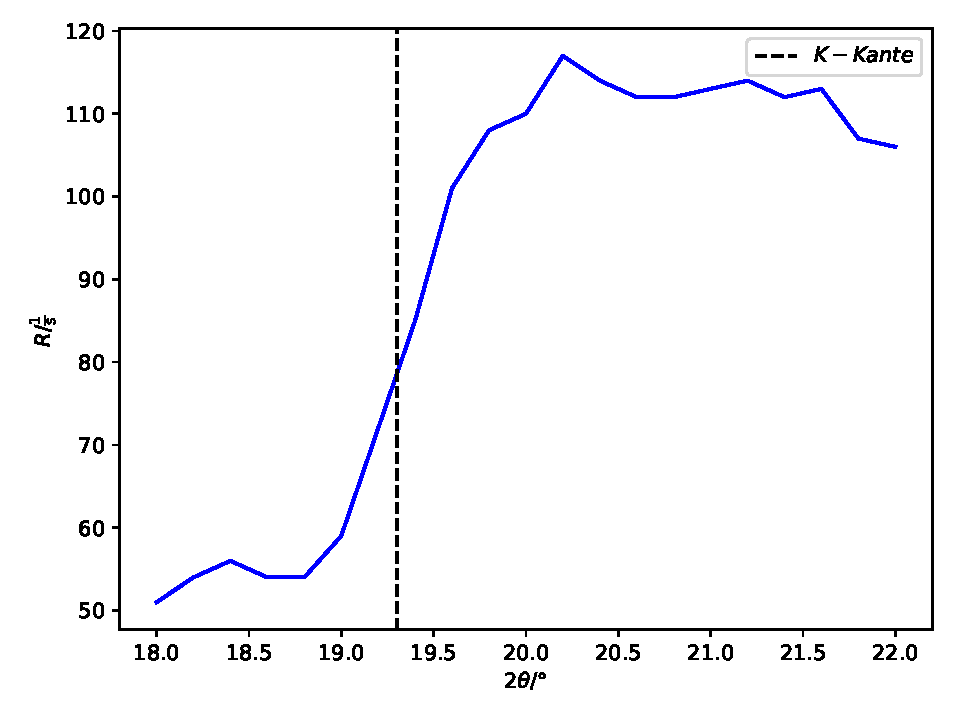
\includegraphics[scale=0.7]{Zirkonium.pdf}
  \caption{Absorptionsspektrum von Zirconium, Rate $R$.}
  \label{abb:zirconium} %Zirconium
\end{figure}
\begin{figure}
  \centering
  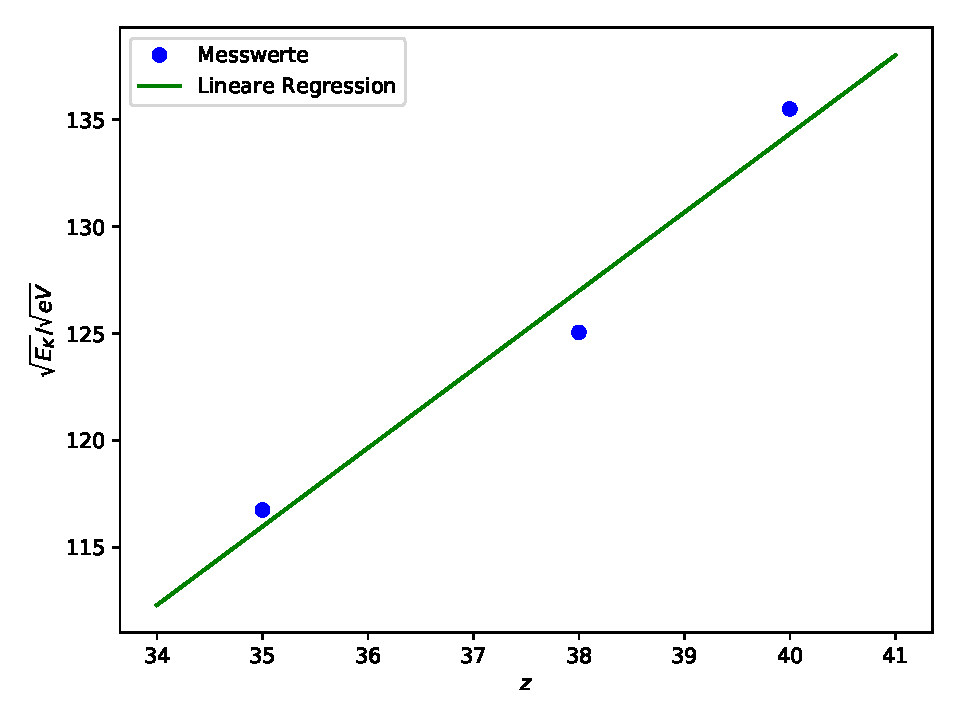
\includegraphics[scale=0.7]{Lineare Regression.pdf}
  \caption{Lineare Regression.}
  \label{abb:lineare_Regression} %Lineare Regression %lineare REgression
\end{figure}
\begin{table}
  \centering
  \caption{Messwerte zum Spektrum leichter Elemente, Rate $R$.}
  \label{tab:leichteElemente}
  \begin{tabular}{c c | c c | c c}
    \toprule
    \multicolumn{2}{c}{Brom} & \multicolumn{2}{c}{Strontium} & \multicolumn{2}{c}{Zirconium} \\
    $\theta$ / $\si{\degree}$ & $R$ / $\si{\per\second}$ & $\theta$ / $\si{\degree}$ & $R$ / $\si{\per\second}$ & $\theta$ / $\si{\degree}$ & $R$ / $\si{\per\second}$ \\
    \midrule
    24.00 & 10.00 & 19.00 & 27.00 & 18.00 & 51.00 \\
    24.20 & 11.00 & 19.20 & 29.00 & 18.20 & 54.00 \\
    24.40 & 11.00 & 19.40 & 28.00 & 18.40 & 56.00 \\
    24.60 & 10.00 & 19.60 & 27.00 & 18.60 & 54.00 \\
    24.80 & 9.00 & 19.80 & 27.00 & 18.80 & 54.00 \\
    25.00 & 9.00 & 20.00 & 28.00 & 19.00 & 59.00 \\
    25.20 & 9.00 & 20.20 & 27.00 & 19.20 & 72.00 \\
    25.40 & 8.00 & 20.40 & 27.00 & 19.40 & 85.00 \\
    25.60 & 9.00 & 20.60 & 26.00 & 19.60 & 101.00 \\
    25.80 & 11.00 & 20.80 & 24.00 & 19.80 & 108.00 \\
    26.00 & 12.00 & 21.00 & 25.00 & 20.00 & 110.00 \\
    26.20 & 18.00 & 21.20 & 28.00 & 20.20 & 117.00 \\
    26.40 & 19.00 & 21.40 & 33.00 & 20.40 & 114.00 \\
    26.60 & 22.00 & 21.60 & 46.00 & 20.60 & 112.00 \\
    26.80 & 21.00 & 21.80 & 58.00 & 20.80 & 112.00 \\
    27.00 & 19.00 & 22.00 & 68.00 & 21.00 & 113.00 \\
    27.20 & 17.00 & 22.20 & 73.00 & 21.20 & 114.00 \\
    27.40 & 17.00 & 22.40 & 71.00 & 21.40 & 112.00 \\
    27.60 & 17.00 & 22.60 & 75.00 & 21.60 & 113.00 \\
    27.80 & 15.00 & 22.80 & 72.00 & 21.80 & 107.00 \\
    28.00 & 17.00 & 23.00 & 70.00 & 22.00 & 106.00 \\
    28.20 & 17.00 & 23.20 & 65.00 & & \\
    28.40 & 16.00 & 23.40 & 65.00 & & \\
    28.60 & 15.00 & 23.60 & 68.00 & & \\
    28.80 & 15.00 & 23.80 & 66.00 & & \\
    29.00 & 14.00 & 24.00 & 64.00 & & \\
    29.20 & 14.00 & 24.20 & 66.00 & & \\
    29.40 & 13.00 & 24.40 & 64.00 & & \\
    29.60 & 14.00 & 24.60 & 63.00 & & \\
    29.80 & 13.00 & 24.80 & 56.00 & & \\
    30.00 & 11.00 & 25.00 & 56.00 & & \\
    \bottomrule
  \end{tabular} %Tabelle Brom, Strontium, Zirconium
\end{table}


\subsection{Absorptionsspektrum von Quecksilber}

Um die Absorptionskonstante von der L-Kante von Quecksilber zu bestimmen wird die Formel \eqref{eq:quecksilber} verwendet.
Hierzu muss zunächst $\Delta E$ an dem Graphen abgelesen werden, hierzu werden die Winkel der Kanten bestimmt und mit Hilfe
der Formel \eqref{eq:energie} die zugehörigen Energien bestimmt.
\begin{align*}
  \theta_{\symup{L2}} &= \SI{12,5}{\degree} \\
  \theta_{\symup{L3}} &= \SI{14,5}{\degree} \\
  E_{\symup{\theta_{\symup{L2}}}} &= \SI{14,221}{\kilo\eV} \\
  E_{\symup{\theta_{\symup{L3}}}} &= \SI{12,294}{\kilo\eV} \\
  \Delta E &= \SI{1,928}{\kilo\eV}
\end{align*}
Mit der Formel \ref{eq:quecksilber} lässt sich nun die Abschirmkonstante $\sigma_L$ Berechnungen
\begin{equation}
  \sigma_L = 3,569
\end{equation}
\begin{table}
  \centering
  \caption{Messwerte zur Messung des Spektrums von Quecksilber, Rate $R$.}
  \label{tab:quecksilber}
  \begin{tabular}{c c | c c }
    \toprule
    $\theta$ / $\si{\degree}$ & $R$ / $\si{\per\second}$ & $\theta$ / $\si{\degree}$ & $R$ / $\si{\per\second}$ \\
    \midrule
    22.00 & 21.00 & 27.20 & 14.00 \\
    22.20 & 19.00 & 27.40 & 14.00 \\
    22.40 & 22.00 & 27.60 & 15.00 \\
    22.60 & 21.00 & 27.80 & 14.00 \\
    22.80 & 21.00 & 28.00 & 13.00 \\
    23.00 & 21.00 & 28.20 & 16.00 \\
    23.20 & 18.00 & 28.40 & 14.00 \\
    23.40 & 19.00 & 28.60 & 16.00 \\
    23.60 & 21.00 & 28.80 & 19.00 \\
    23.80 & 20.00 & 29.00 & 24.00 \\
    24.00 & 20.00 & 29.20 & 24.00 \\
    24.20 & 20.00 & 29.40 & 22.00 \\
    24.40 & 19.00 & 29.60 & 21.00 \\
    24.60 & 20.00 & 29.80 & 22.00 \\
    24.80 & 22.00 & 30.00 & 20.00 \\
    25.00 & 23.00 & 30.20 & 20.00 \\
    25.20 & 23.00 & 30.40 & 19.00 \\
    25.40 & 21.00 & 30.60 & 18.00 \\
    25.60 & 21.00 & 30.80 & 18.00 \\
    25.80 & 21.00 & 31.00 & 18.00 \\
    26.00 & 18.00 & 31.20 & 17.00 \\
    26.20 & 18.00 & 31.40 & 15.00 \\
    26.40 & 17.00 & 31.60 & 17.00 \\
    26.60 & 16.00 & 31.80 & 16.00 \\
    26.80 & 18.00 & 32.00 & 15.00 \\
    27.0 &	15.0 & & \\
    \bottomrule
  \end{tabular} %Tabelle Quecksilber
\end{table}
\begin{figure}
  \centering
  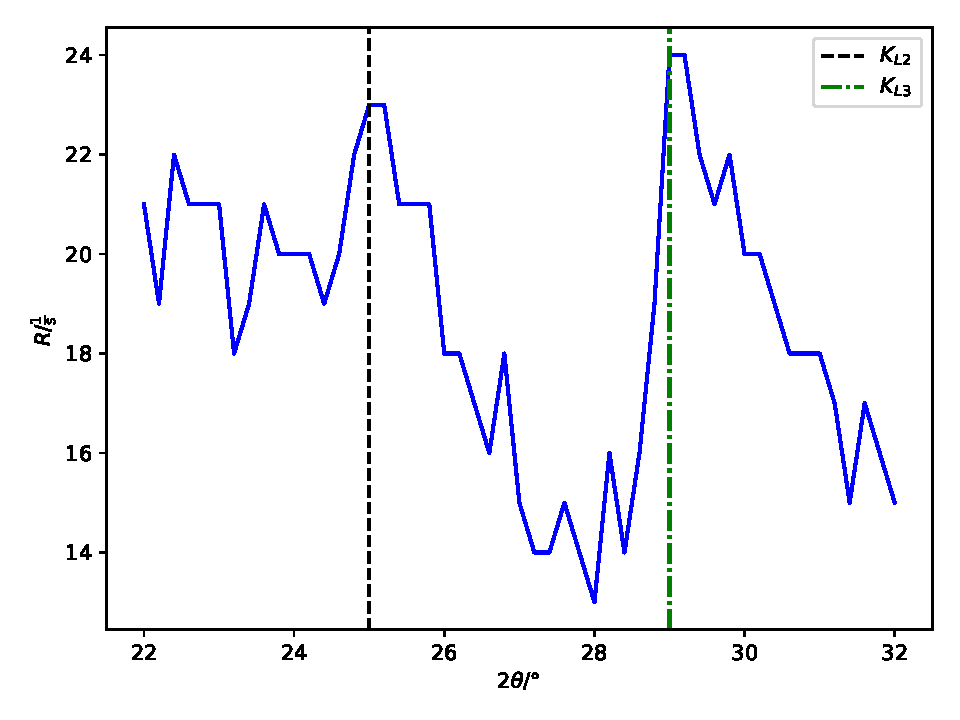
\includegraphics[scale=0.7]{Quecksilber.pdf}
  \caption{Absorptionsspektrum von Quecksilber, Rate $R$.}
  \label{abb:quecksilber} %Quecksilber
\end{figure}

\section{Diskussion}
Im ersten Teil des Versuchs sollte die Braggbedingung überprüft werden, hierbei wurde ein Winkel von
$\theta_{\symup{gemessen}}=\SI{14,2}{\degree}$ gemessen, der LIteraturwert ist $\theta_{\symup{Literatur}}=\SI{14}{\degree}$.
Die Abweichung vom Literaturwert beträgt $\SI{1,43}{\percent}$.

Im zweiten Teil des Versuchs sollte das Emissionsspektrum einer Cu-Röntgenröhre untersucht werden. Hierbei wurde die maximale Energie
berechnet mit $E_{\symup{max gemessen}} = \SI{35,317}{\kilo\eV}$, der Literaturwert besagt $E_{\symup{max Literatur}} = \SI{35}{\kilo\eV}$.
Die relative Abweichung von $\SI{0,91}{\percent}$ lässt sich durch das ungenaue Ablesen des Winkels aus dem Plot erklären. Außerdem
sollte zusätzlich der Absorptionskoeffizient berechnet werden.
\begin{align*}
  \sigma_{K gemessen} = 13,159 \\
  \sigma_{K Literatur} = 13,03
\end{align*}
Die Abweichung von $\SI{0,99}{\percent}$ lässt sich erneut auf das Ablesen der Werte aus dem Graphen bzw. aus der Tabelle ablesen.
Außerdem wird der Peak von nur etwas 5-6 Messwerten beschrieben, da kann es zu geringen Verschiebungen des Maximums führen, die sich widerum auf
die Energien und somit auf den Absorptionskoeffizienten auswirken.

Im letzten Teil des Versuchs sollen verschiedene Absorptionskoeffizienten von verschiedenen Stoffen berechnet werden. Die
Literaturwerte, die gemessenen Werte und die Abweichungen sind in Tabelle \ref{tab:diskussion} aufgelistet. Die Abweichungen lassen sich erneut
auf das Ablesen der Werte aus den Plots zurück führen. Hierbei wurde der Winkel von der Mitte der Kante genommen. Die berechneten Energien
der K-Kante werden in Tabelle \ref{tab:energie} verglichen.

\begin{table}
  \centering
  \caption{Absoptionskoeffizienten und Abweichungen.}
  \label{tab:diskussion}
  \begin{tabular}{c | c c | c}
    \toprule
    & $\sigma_{\symup{K gemessen}}$ & $\sigma_{\symup{K Literatur}}$ & Abweichung / $\si{\percent}$ \\
    \midrule
    Brom & 3,340 & 3,85 & \SI{13,24}{\percent} \\
    Strontium & 4,088 & 4,00 & \SI{2,20}{\percent} \\
    Zirconium & 3,255 & 4,10 & \SI{20,61}{\percent} \\
    \bottomrule
  \end{tabular}
\end{table}

\begin{table}
  \centering
  \caption{Berechnete Energien, Literaturwerte und Abweichungen.}
  \label{tab:energie}
  \begin{tabular}{c | c c | c}
    \toprule
    & $E_{\symup{K gemessen}}$ / $\si{\kilo\eV}$ & $E_{\symup{K Literatur}}$ / $\si{\kilo\eV}$  & Abweichung / $\si{\percent}$ \\
    \midrule
    Brom & 13,632 &  13,48 & 1,13 \\
    Strontium &  15,640 &  16,12 & 3,07 \\
    Zirconium &  18,362 &  18,01 & 1,95 \\
    \bottomrule
  \end{tabular}
\end{table}

\nocite{*}
\printbibliography
